\section{Implementácia algoritmu}
\label{kap:4}

Kým v predošlej kapitole (kap. \ref{kap:3}) sme si v jednoduchosti vysvetlili ako budeme pristupovať ku plánovaniu trajektórie pri jednotlivých kinematických štruktúrach a opísali sme si konfiguračný priestor pre jednotlivé štruktúry, v tejto kapitole si bližšie vysvetlíme, čo bolo potrebné implementovať do pôvodného kódu aby vyššie spomenuté prístupy fungovali.

Ukážeme si fundamentálne funkcie, na ktorých stojí náš algoritmus a vysvetlíme si ich úlohy a prístup, ktorý sme pri ich implementácii zvolili.
 



\subsection{Vizualizácia}

Pre potreby vývoju nášho algoritmu bolo v prvom rade potrebné vytvoriť vizualizáciu prenášaného objektu v priestore. Pôvodné riešenie uvažovalo len hmotný bod, ktorého pohyb v priestore sa dá jednoducho zobraziť v grafe. Pri našom probléme má však prenášaný objekt svoj, tvar, rozmery a orientáciu v priestore. Z toho dôvodu bola vytvorená vizualizácia, ktorá nám zobrazuje priemet pracovného priestoru robota v osiach $ x $, $ y $ (obr. \ref{OBRAZOK 4.1}). Obsahuje prenášaný predmet, prekážku, ktorá predstavuje stĺp, na ktorom je robotické rameno uchytené  v prípade plánovania trajektórie v kĺbovom priestore aj samotné robotické rameno. Pracovný priestor spolu s prekážkami a objektom sme vizualizovali v mierke  1 $mm$ = 1 $pixel$. 

\begin{figure}[h]
	\centering
	\fbox{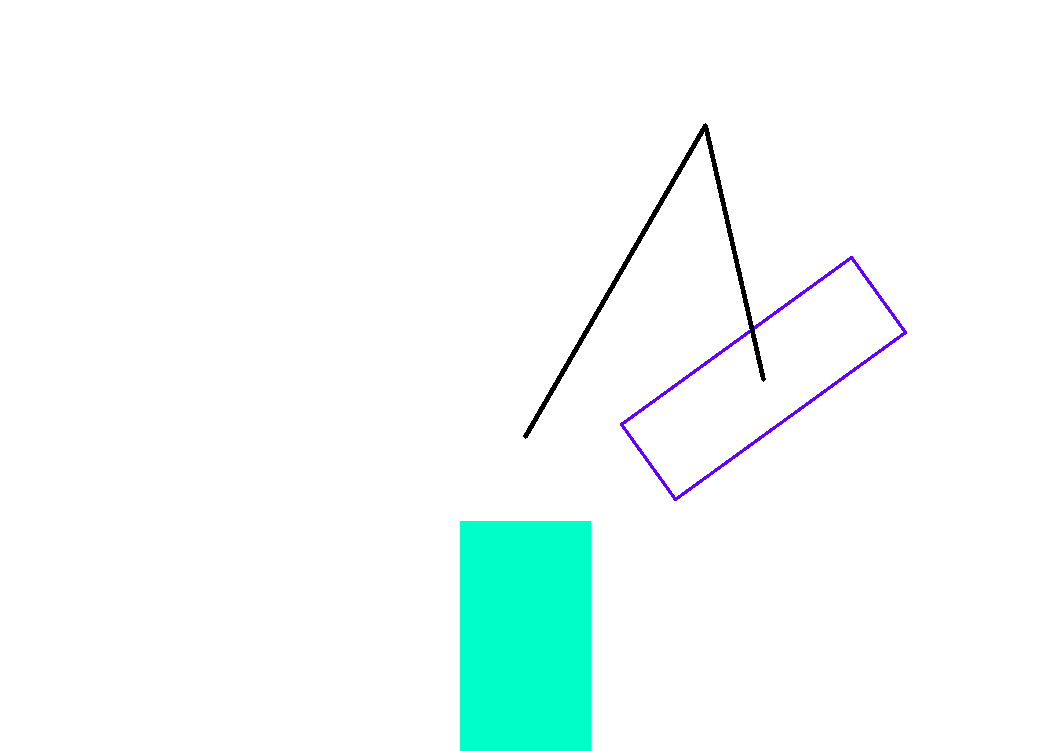
\includegraphics[width=100mm]{img/Vizualizacia.png}}
	\caption{Vizualizácia pracovného priestoru} \label{OBRAZOK 4.1} 
	\label{fig:border}
\end{figure} 

Táto vizualizácia spĺňala v prvom rade kontrolnú funkciu, či vygenerovaná trajektória spĺňa dané požiadavky - sa objekt pri pohybe vyhýba prekážkam a nevychádza z pracovného priestoru.

Prenášaný objekt sme si vizualizovali ako obdĺžnik. Ide o univerzálny geometrický tvar najlepšie odpovedajúci  väčšine tovaru, ktorý by sa mohol v sklade nachádzať. Takmer každá krabička alebo iný objekt sa nám do roviny $ xy $ premietne práve ako obdĺžnik. Objekt sme teda definovali pozíciou jeho stredu, výškou, šírkou a uhlom otočenia. 

Pre vypracovanie tejto časti sme využili knižnicu openCV.

\subsection{Objekt v kolízii}
Hmotný bod prenášaný priestorom má v porovnaní s objektom veľkú výhodu práve v tom, že vieme presne povedať kde v priestore sa nachádza. Tým pádom vieme jednoducho určiť , či je v kolízii s prekážkami alebo opustil pracovný priestor. Pri objekte vieme takýmto spôsobom kontrolovať len jeden jeho bod, ktorým je definovaný a to je v našom prípade jeho stred. Úlohu kontroly kolízie objektu s prekážkami to teda výrazne komplikuje aj vzhľadom na to, že náš objekt mení v priestore aj svoju orientáciu. 

Preto bolo potrebné vytvoriť funkciu, ktorej úlohou bude zistiť či sa náš objekt v danej konfigurácii nenachádza v kolízii alebo neopustil pracovný priestor robota. Touto funkciou je $ collision\_check() $. Ide o základnú funkciu na ktorej stojí celý náš algoritmus a je identická pre všetky kinematické štruktúry. Pracuje v kartézskom súradnicovom systéme. Na základe vstupných údajov, ktorými sú pozícia stredu objektu - súradnice $ x $ a $ y $, rozmery objektu - šírka a výška, a natočenie objektu nám vráti informáciu o tom či sa objekt nachádza v bezkolíznej pozícii. 

\begin{figure}[h!]
	\centering
	\fbox{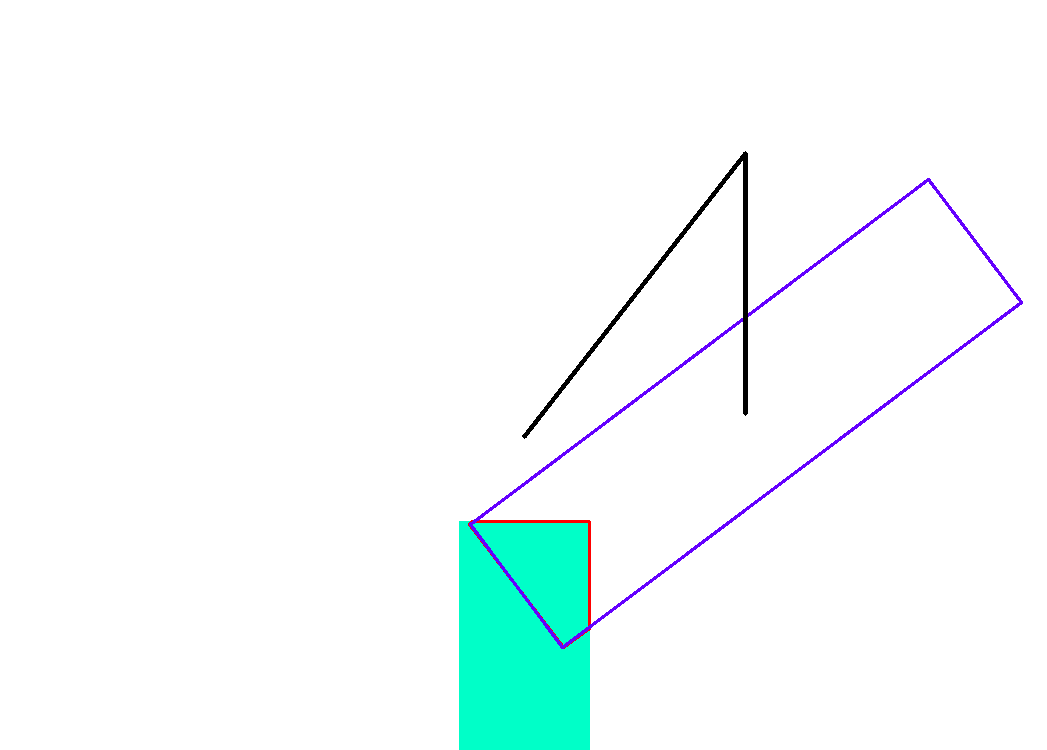
\includegraphics[width=100mm]{img/Kolizia.png}}
	\caption{Objekt v kolízii} \label{OBRAZOK 4.2} 
\end{figure} 

Pre kontrolu kolízie objektu s prekážkami v priestore sme použili knižnicu shapely. Pomocou jej funkcií sme boli schopní na základe parametrov objektu získať pozíciu jeho rohov v priestore a tiež overiť prienik 2 objektov - prenášaného a prekážky, čo nám slúžilo na zistenie kolízie(obr. \ref{OBRAZOK 4.2} ).

Do tejto funkcie sme zahrnuli kontrolu situácie, že prenášaný objekt opustí pracovný priestor robota. Keďže nevieme zaručiť, že priestor mimo pracovné priestoru robota bude voľný, treba ho považovať za obsadený. V prípade, že objekt opusti pracovný priestor je táto konfigurácie tiež považovaná za kolíziu. 
 
\subsection{Overenie dosiahnuteľnosti pozície}

Generovanie trajektórie prebieha v krokoch, kedy sú postupne generované nové konfigurácie alebo inak povedané pozície, ktorými objekt prechádza od počiatku k cieľu (kapitola \ref{kap:2.1}). Prvým krokom je určiť, či sa vygenerovaný nachádza v bezkolíznej konfigurácii, k čomu slúži funkcia $ collision\_check() $. Druhým krokom je zistiť, či sa objekt z bodu, v ktorom sa práve nachádza dokáže dostať do nového bodu, ktorý bol vygenerovaný. Ak by ho objekt z danej pozície nemohol dosiahnuť napr. kvôli prekážke v ceste, tento bod nemôže byť pridaný do generovaného stromu. V prípade hmotného bodu ide o priame spojenie 2 bodov priamkou. Ak sa priamka pretína s prekážkou tak táto pozícia nie je dosiahnuteľná. 

Pri objekte treba uvažovať jeho pohyb v priestore.  Každá pozícia, ktorou objekt pri danom pohybe prejde musí byť bezkolízna. Na obrázkoch \ref{OBRAZOK 4.4} a \ref{OBRAZOK 4.5} môžeme vidieť porovnanie medzi pracovným a konfiguračným priestorom.  Kým v konfiguračnom priestore je pohyb opísaný priamkou v trojrozmernom priestore, v pracovnom priestore ide o pohyb obdĺžnika, kedy sa menia jeho pozícia v osiach $ x $, $ y $ aj uhol natočenia.

\begin{figure}[h!]
	\centering
	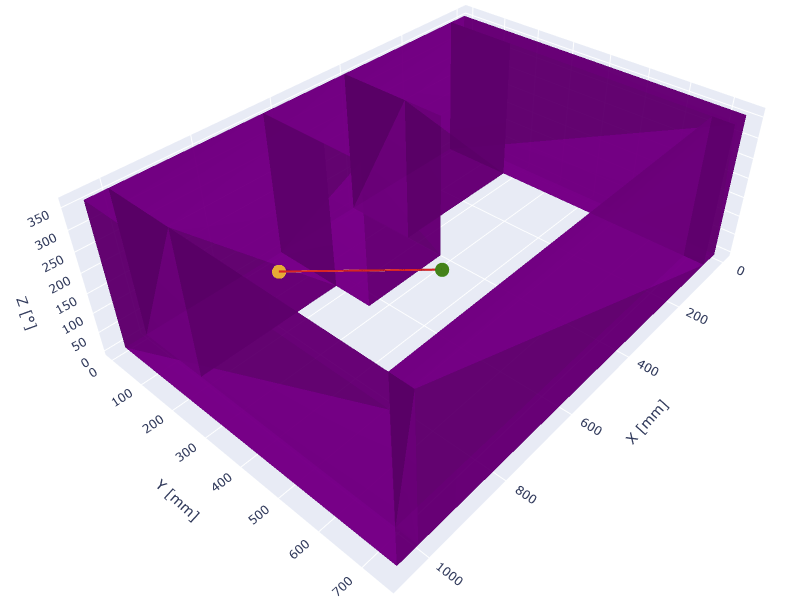
\includegraphics[width=120mm]{img/Path_sampling-Searchspace.png}
	\caption{Spojenie 2 bodov v konfiguračnom priestore} \label{OBRAZOK 4.4} 
\end{figure} 

\begin{figure}[h!]
	\centering
	\fbox{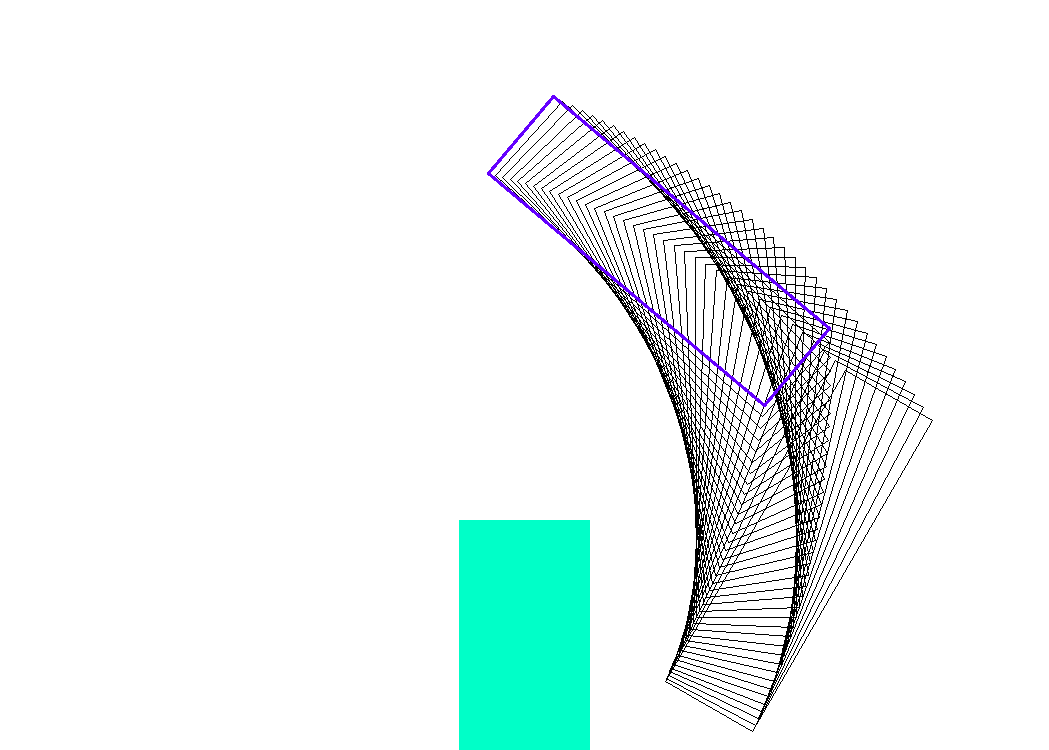
\includegraphics[width=100mm]{img/Path_sampling3D.png}}
	\caption{Pohyb objektu v pracovnom priestore} \label{OBRAZOK 4.5} 
\end{figure} 


Pre simuláciu pohybu v priestore sme použili lineárne vzorkovania. Poznáme počiatočnú a koncovú pozíciu, ktoré nám definujú pohyb - prejdenú vzdialenosť a smer. Vypočítame si veľkosť úsečky medzi danými 2 pozíciami v konfiguračnom priestore. Na základe nami zvolenej veľkosti vzorky si rozdelím danú uhlopriečku na daný počet vzoriek. Postupne inkrementujeme jednotlivé prvky počiatočnej pozície ($ x $,$ y $,$ uhol $) o hodnotu, ktorá odpovedá veľkosti vzorky v danej osi. Tým dosiahneme prechodové pozície, pričom v každej z nich kontrolujeme, či sa objekt nenachádza v kolízii.  Ak sú všetky prechodové pozície vyhodnotené ako bezkolízne vieme, že daný cieľový bod je dosiahnuteľný.
Túto úlohu zabezpečuje funkcia $ linear\_sampling\_collision\_check()$.

OBRAZOK - linearne vzorkovanie


\subsection{Kontrola dosiahnuteľnosti cieľa}

Ukončovacia podmienka algoritmu býva vo väčšine prípadov určená vzdialenosťou generovaného bodu v strome od cieľovej pozície, keď sa generovaný bod dostane do blízkosti cieľa je vytvorené prepojenie a algoritmus je ukončený. Ďalšou možnosťou je použiť ako ukončovacia podmienku maximálny počet iterácií. Algoritmus prehľadáva priestor až dokým nie je vygenerovaný daný počet bodov a až následne hľadá prepojenie s cieľom. Táto ukončovacia podmienka sa dá použiť napríklad pri RRT*, kedy je počtu iterácií úmerná kvalita výslednej trajektórie. Pri algoritme RRT-connect sú generované 2 stromy a ukončenie algoritmu
nastane pri ich spojení.

V našom algoritme využíva určitú kombináciu jednotlivých prístupov.
Jedným so vstupných parametrov, ktorý si definujeme pri spustení algoritmu je pravdepodobnosť, s ktorou si bude algoritmus v priebehu generovania stromu kontrolovať dosiahnuteľnosť cieľa.  V prípade, že je cieľ z daného bodu dosiahnuteľný je vygenerovaná trajektória a algoritmus je ukončený. Na kontrolu dosiahnuteľnosti cieľa z posledného generovaného bodu nám slúži funkcia $ linear\_sampling\_collision\_check()$.

Z dôvodu jednoduchosti pracovného priestoru (obsahuje len jednu prekážku) vo väčšine prípadov prenášaných objektov bude možné nájsť priame spojenie hneď z počiatočnej do cieľovej pozície. Za účelom zvýšenia rýchlosti výpočtu algoritmu v daných prípadoch si algoritmus hneď na začiatku skontroluje dosiahnuteľnosť cieľa, čím sa preskočí celý proces generovania stromu.

Algoritmu je tiež stanovený maximálny počet iterácií. V prípade dosiahnutia maximálneho počtu iterácií je overená dosiahnuteľnosť cieľa z daného bodu. Ak spojenie neexistuje algoritmus je ukončený a trajektória nebola nájdená.

\subsection{3 stupne voľnosti}

Plánovanie trajektórie objektu pri troch stupňoch voľnosti ponúka väčšie možnosti pohybu v priestore, väčšiu množinu potenciálnych pozícií, do ktorých sa môže teleso dostať. Hlavný rozdiel je v treťom kĺbe, ktorý poskytuje možnosť otáčať objektom v jeho danej pozícii a tým sa vyhýbať kolíziám s prekážkami a vyjdeniu z pracovného priestoru. Plánovanie bude prebiehať v kartézskom aj kĺbovom súradnicovom systéme. Program je potrebné prispôsobiť pre oba prípady zvlásť, každý si vyžaduje iné prístupy a úpravy, keďže každý súradnicový systém má svoje vlastné charakteristiky a obmedzenia

\subsubsection{Kartézsky súradnicový systém}

Plánovanie v kartézskom súradnicovom systéme je z programovej stránky najjednoduchšie riešenie, ktoré sme implementovali. 
Ide o pôvodné riešenie rozšírené len o už spomenuté funkcie $ collision\_check() $ a $ linear\_sampling\_collision\_check()$. Princíp fungovania môžeme vidieť na obrázku \ref{OBRAZOK 4.16}.


 \begin{figure}[h!]
	\centering
	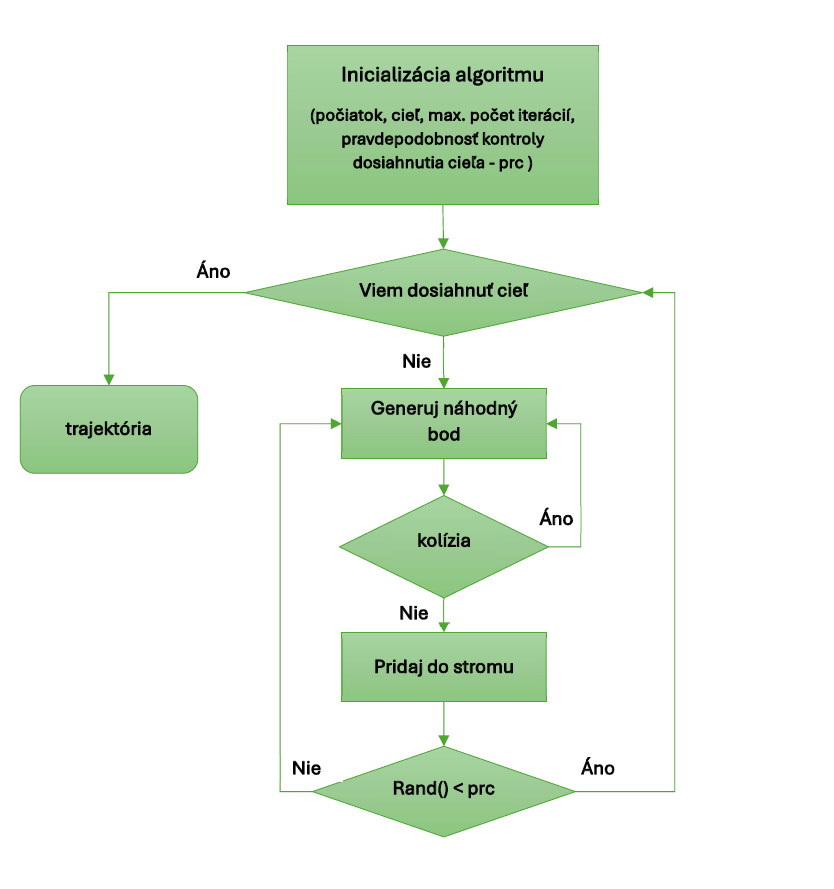
\includegraphics[width=140mm]{img/VD_RRT.png}
	\caption{RRT algoritmus} \label{OBRAZOK 4.16} 
\end{figure}

 
 Za účelom zrýchlenia algoritmu sme sa rozhodli o jednoduché obmedzenie konfiguračného priestoru. To sme implementovali tak, že sme vytvorili prekážky v konfiguráciách o ktorých sme si istý že objekt nemôže dosiahnuť alebo nechceme aby sa strom rozvíjal daným smerom. Pre toto obmedzenie je potrebné poznať rozmery objektu. Porovnáme si jeho šírku a výšku a vyberieme si jeho menší rozmer. O tento rozmer rozšírime hranice konfiguračného priestoru v osiach $ x $ a $ y $ a všetky možné rotácie v daných bodoch. Výsledok obmedzenia konfiguračného priestoru môžeme vidieť na obrázku . Výsledkom je zrýchlenie algoritmu keďže nie sú generované nové pozície v daných kolíznych konfiguráciách a algoritmus má tendenciu hľadať bližšie v okolí cieľovej pozície. Toto obmedzenie nám pomôže hlavne v situáciách ak sa jedná o objekt väčších rozmerov. 
 
  \begin{figure}[h!]
 	\centering
 	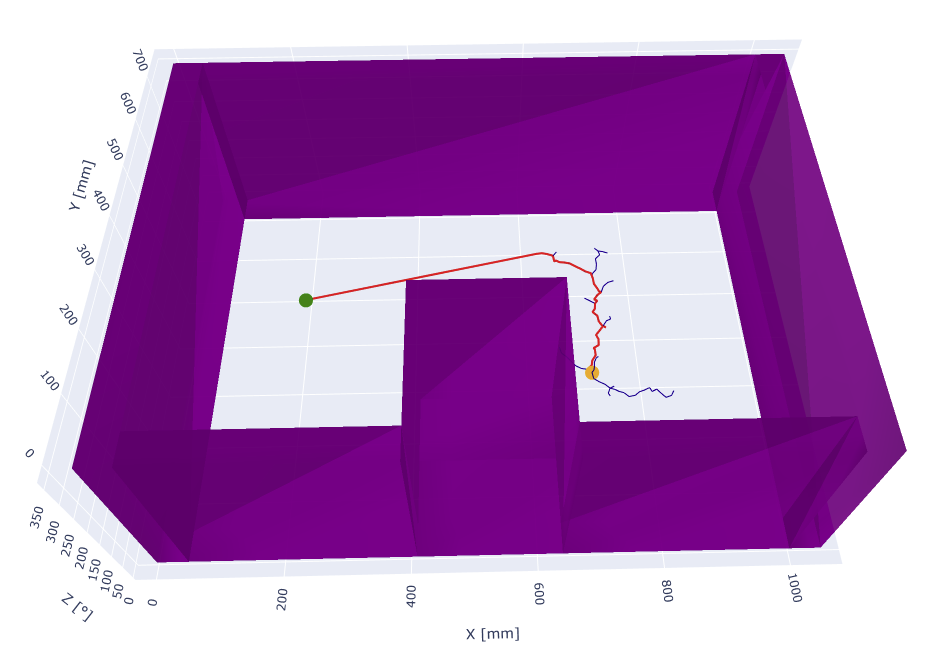
\includegraphics[width=100mm]{img/ObmedzenieCfree.png}
 	\caption{Obmedzenie konfiguračného priestoru} \label{OBRAZOK 4.6} 
 \end{figure}
 
\subsubsection{Kĺbový súradnicový systém}

Použitie kĺbového súradnicového systému ako konfiguračného priestoru pre plánovanie trajektórie so sebou prináša určité výhody. Hlavnou výhodou je väčšia pravdepodobnosť nájdenia priameho spojenia z počiatočného bodu do cieľovej pozície. Situácie kedy sa v kartézskom systéme nachádza medzi počiatkom a cieľom prekážka sa do kĺbového súradnicového systému premietne iným spôsobom. Tu je možné nájsť priame bezkolízne spojenie medzi danými 2 bodmi keďže priamy pohyb v kĺbovom priestore sa v kartézskom zobrazí ako pohyb po kružnici (obr. \ref{OBRAZOK 4.7}). 

 \begin{figure}[h!]
 	\centering
 	\fbox{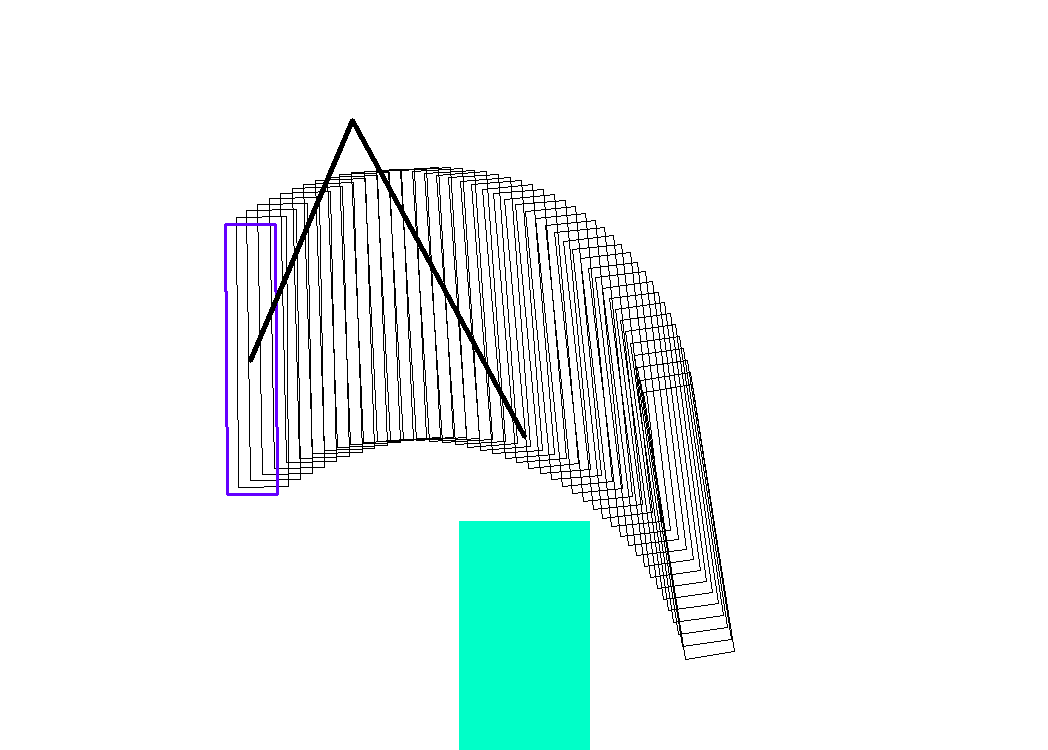
\includegraphics[width=100mm]{img/3DOF_Q_obidenie_prekazky.png}}
 	\caption{Pohyb objektu v pracovnom priestore} \label{OBRAZOK 4.7} 
 \end{figure} 

Z dôvodu odlišnosti medzi konfiguračným a pracovným priestorom, keďže každý využíva iný súradnicový systém bolo potrebné implementovať funkcie, ktoré by zabezpečili prechod z jedného do druhého.   

Pre tieto potreby bolo potrebné implementovať funkcie na výpočet priamej a inverznej kinematiky.
Počiatočná a koncová pozícia sú v úlohe definované v pracovnom priestore (kartézsky súradnicový systém). Na ich prepočet do kĺbového systému je použitá inverzná kinematika, ktorej výstupom sú natočenia jednotlivých kĺbov v daných pozíciach. Použitie funkcie  $ collision\_check() $ si vyžaduje aby boli známe súradnice stredu objektu v pracovnom priestore. Z toho dôvodu je potrebný výpočet pozície koncového efektora ramena pomocou priamej kinematiky z kĺbových súradníc daného bodu.

Funkcie na výpočet priamej a inverznej kinematiky sme si implementovali sami. Nebolo potrebné používať žiadnu knižnicu keďže sa jedná len o jednoduché rameno s 3 kĺbmi umiestnenými v jednej rovine. Funkcie bolo možné vytvoriť pomocou jednoduchých vzorcov.

 \begin{figure}[h]
	\centering
	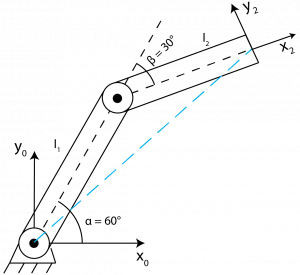
\includegraphics[width=80mm]{img/FK1.png}
	\caption{Robotické rameno s dvoma stupňami voľnosti \cite{FKIK}} \label{OBRAZOK 4.8} 
\end{figure} 

Priama kinematika slúži na získanie súradníc pozície koncového bodu robotického ramena na základe natočenia kĺbov ramena (obr. \ref{OBRAZOK 4.8}). Na výpočet koncovej pozície nám stačí poznať hodnoty natočenia prvého a druhého kĺba. Tretí kĺb sa nachádza v koncovom bode ramena a preto jeho rotácia neovplyvňuje pozíciu koncového bodu.
Tú získame pomocou nasledovných rovníc  \ref{e1}  a  \ref{e2}  \cite{FKIK}.

\begin{equation}
	\begin{aligned}
		x'&= l_1 cos \alpha \\
		x''&= l_2 cos (\alpha + \beta) \\
		y'&= l_1 sin \alpha \\
		y''&= l_2 sin (\alpha + \beta) \\
	\end{aligned}
 \label{e1} 
\end{equation}

\begin{figure}[h]
	\centering
	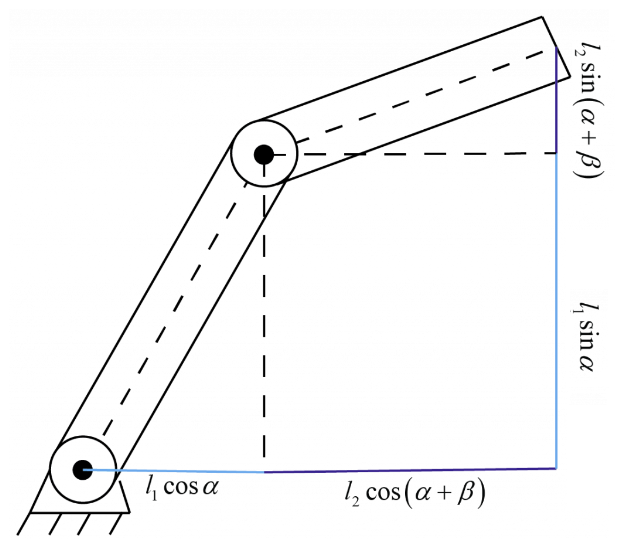
\includegraphics[width=85mm]{img/FK2.png}
	\caption{Súradnice koncového bodu \cite{FKIK} } \label{OBRAZOK 4.9} 
\end{figure} 

\begin{equation}
	\begin{aligned}
		x&= l_1 cos \alpha + l_2 cos (\alpha + \beta) \\
		y&= l_1 sin \alpha +  l_2 sin (\alpha + \beta) \\
	\end{aligned}
 \label{e2} 
\end{equation}

Pri priamej kinematike je tiež dôležité nezabudnúť že od natočenia prvých dvoch kĺbov je závislá orientácia koncového efektora, v ktorom je umiestnený tretí kĺb. Teda orientácia uchyteného objektu sa bude meniť aj bez rotácie tretieho kĺba, ten naopak túto rotáciu dokáže vyrovnávať v rámci rozsahu svojho pohybu. Natočenie koncového efektora získame ako súčet hodnôt prvého a druhého kĺba (rovnica  \ref{e5}).

\begin{equation}
	uhol=\alpha + \beta \\
	\label{e5} 
\end{equation}

Inverzná kinematika, ako vyplýva z názvu, spĺňa opačný účel ako priama kinematika. Na základe súradníc koncového bodu robota získame natočenia kĺbov robota. Pre každú pozíciu však existujú potenciálne 2 riešenia - s kĺbom hore a kĺbom dole (obr. \ref{OBRAZOK 4.10}). 

\begin{figure}[h]
	\centering
	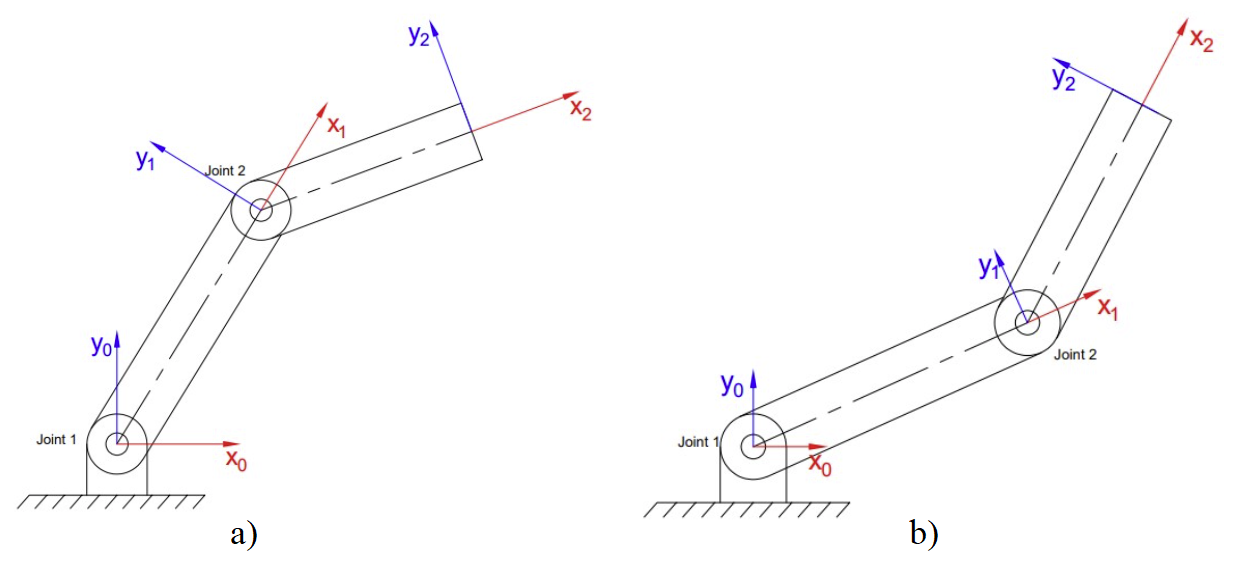
\includegraphics[width=140mm]{img/IK-EUED.png}
	\caption{Dve možné riešenia \cite{FKIK}} \label{OBRAZOK 4.10} 
\end{figure} 

Výpočet inverznej kinematiky robíme pomocou rovníc  \ref{e3 - dole} pre kĺb dole  a rovníc \ref{e4 - hore} pre riešenie s kĺbom hore  \cite{prezentacia}.

\begin{figure}[h]
	\centering
	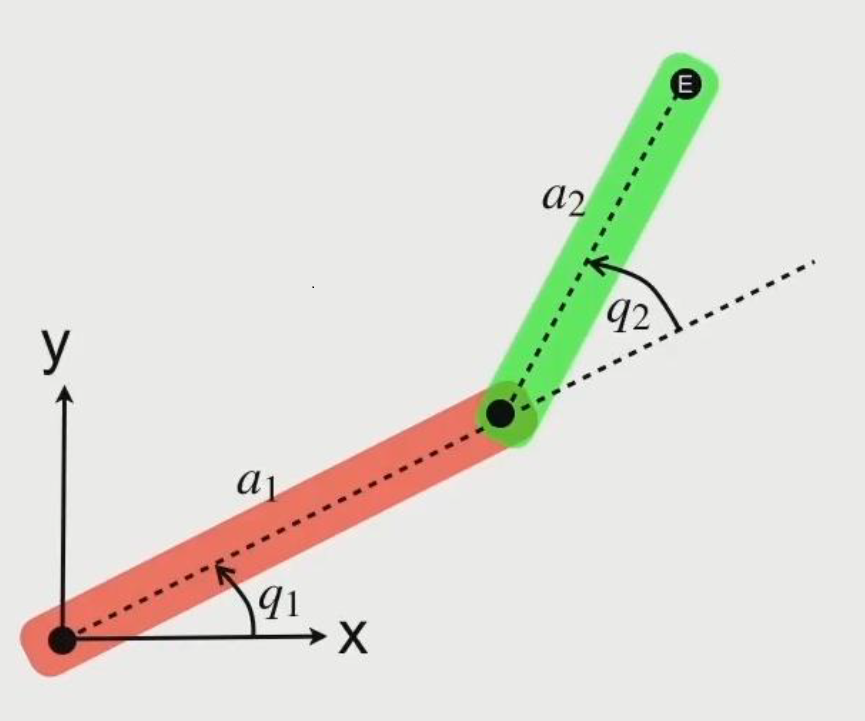
\includegraphics[width=80mm]{img/IK1.png}
	\caption{ Inverzná kinematika - kĺb dole \cite{prezentacia}} \label{OBRAZOK 4.11} 
\end{figure} 

\begin{equation}
	\begin{aligned}
		q_2&= cos^{-1} \frac{x^2 + y^2 - a_1^2 - a_2^2}{2 a_1 a_2 }\\
		q_1&=  tan^{-1} \frac{y}{x} - tan^{-1} \frac{a_2 sinq_2}{a_1 + a_2 cos q_2} \\
	\end{aligned}
	\label{e3 - dole} 
\end{equation}

\begin{equation}
	\begin{aligned}
		q_2&= - cos^{-1} \frac{x^2 + y^2 - a_1^2 - a_2^2}{2 a_1 a_2 }\\
		q_1&=  tan^{-1} \frac{y}{x} + tan^{-1} \frac{a_2 sinq_2}{a_1 + a_2 cos q_2} \\
	\end{aligned}
	\label{e4 - hore} 
\end{equation}


Nevýhodou kĺbového súradnicové systému v porovnaní s kartézskym je obtiažnosť obmedzenia konfiguračného priestoru. Kým v kartézskom systéme sme vedeli jednoducho konfiguračný priestor obmedziť o polohy, do ktorých sa objekt určite nedostane v kĺbovom systéme je táto úloha zložitejšia keďže nevieme jasne určiť, ktoré natočenia kĺbov budú pre danej veľkosti objektu v kolízii. Tým sa nám konfiguračný priestor zväčší aj o kolízne pozície, ktoré nie je možné identifikovať iným spôsobom ako pomocou funkcie $ collision\_check() $. To má za následok nárast výpočtového času algoritmu.

\subsection{2 stupne voľnosti}

Plánovanie trajektórie pre kinematickú štruktúru s dvoma stupňami voľnosti nám už neponúka možnosť výberu konfiguračného priestoru medzi kartézskym a kĺbovým. Vzhľadom k absencii tretieho kĺbu, umiestneného v efektore robotického ramena nie je možné dosiahnuť ľubovoľnú  pozíciu objektu v priestore. Z toho dôvodu je nutné použiť pre plánovanie konfiguračný priestor s kĺbovým súradnicovým systémom. Pôjde o dvojrozmerný konfiguračný priestor kde osi $ x $ a $ y $ predstavujú natočenia jednotlivých kĺbov $ q1 $ a $ q2 $.  

Absencia možnosti otáčať objektom v ľubovolnom bode pracovného priestore značne limituje možnosti plánovacieho algoritmu. Vo väčšine prípadov prenášaných objektov väčších rozmerov algoritmus nebude schopný nájsť riešenie z dôvodu zlej orientácie objektu. Výsledok je teda závislý od orientácia telesa v počiatočnej polohe kde dochádza k uchyteniu objektu. 

Za účelom eliminácie týchto situácií a tak rozšírenia možností danej kinematickej štruktúry sme sa rozhodli implementovať algoritmus, ktorý by nám dovolil zmeniť počiatočnú orientáciu objektu v priestore do takej pozície aby bolo možné nájsť trajektóriu k cieľu. Ide o princíp predrotácie a zabezpečuje ho funkcia $ pre\_rot() $. Pre použitie tohoto princípu bude samozrejme potrebné použiť v koncovom bode ramena ďalší motor, ktorý by túto rotáciu zabezpečil. Išlo by však o motor určený len na polohovanie a nebolo by ho možné riadiť v reálnom čase v procese prenášania objektu. Výhodou by bola nižšia cena nákladov.

Prvým krokom v princípe predrotácie je identifikácia prípadov, v ktorých je potrebné túto funkciu použiť. Pomocou geometrie sme si vypočítali aké musia byť parametre objektu aby bolo nutné použiť predrotáciu. V procese prechodu z počiatocnej do cieľovej pozície nastáva jedna kritická situácia kedy druhé rameno robota musí preniesť objekt okolo stĺpa, na ktorom je upevnený. Tento moment nastáva pri konfigurácii $ q_1 = 90 \degree $ a $ q_2 = 180 \degree $. V prípade, že uhlopriečka objektu je totožná s orientáciou druhého ramena robota, roh objektu sa nachádza v pozícii kedy najviac zasahuje do priestoru. V tomto bode sme vypočítali hraničnú veľkosť uhlopriečky telesa, ktorej hodnota sa rovná $ 370 mm $ (obr. \ref{OBRAZOK 4.12} ). Ak je uhlopriečka telesa menšia ako táto hodnota, nájdenie výsledku nie je závislé od orientácie telesa. Veľkosť uhlopriečky telesa nám teda slúži ako podmienka pre použitie predrotácie.

\begin{figure}[h]
	\centering
	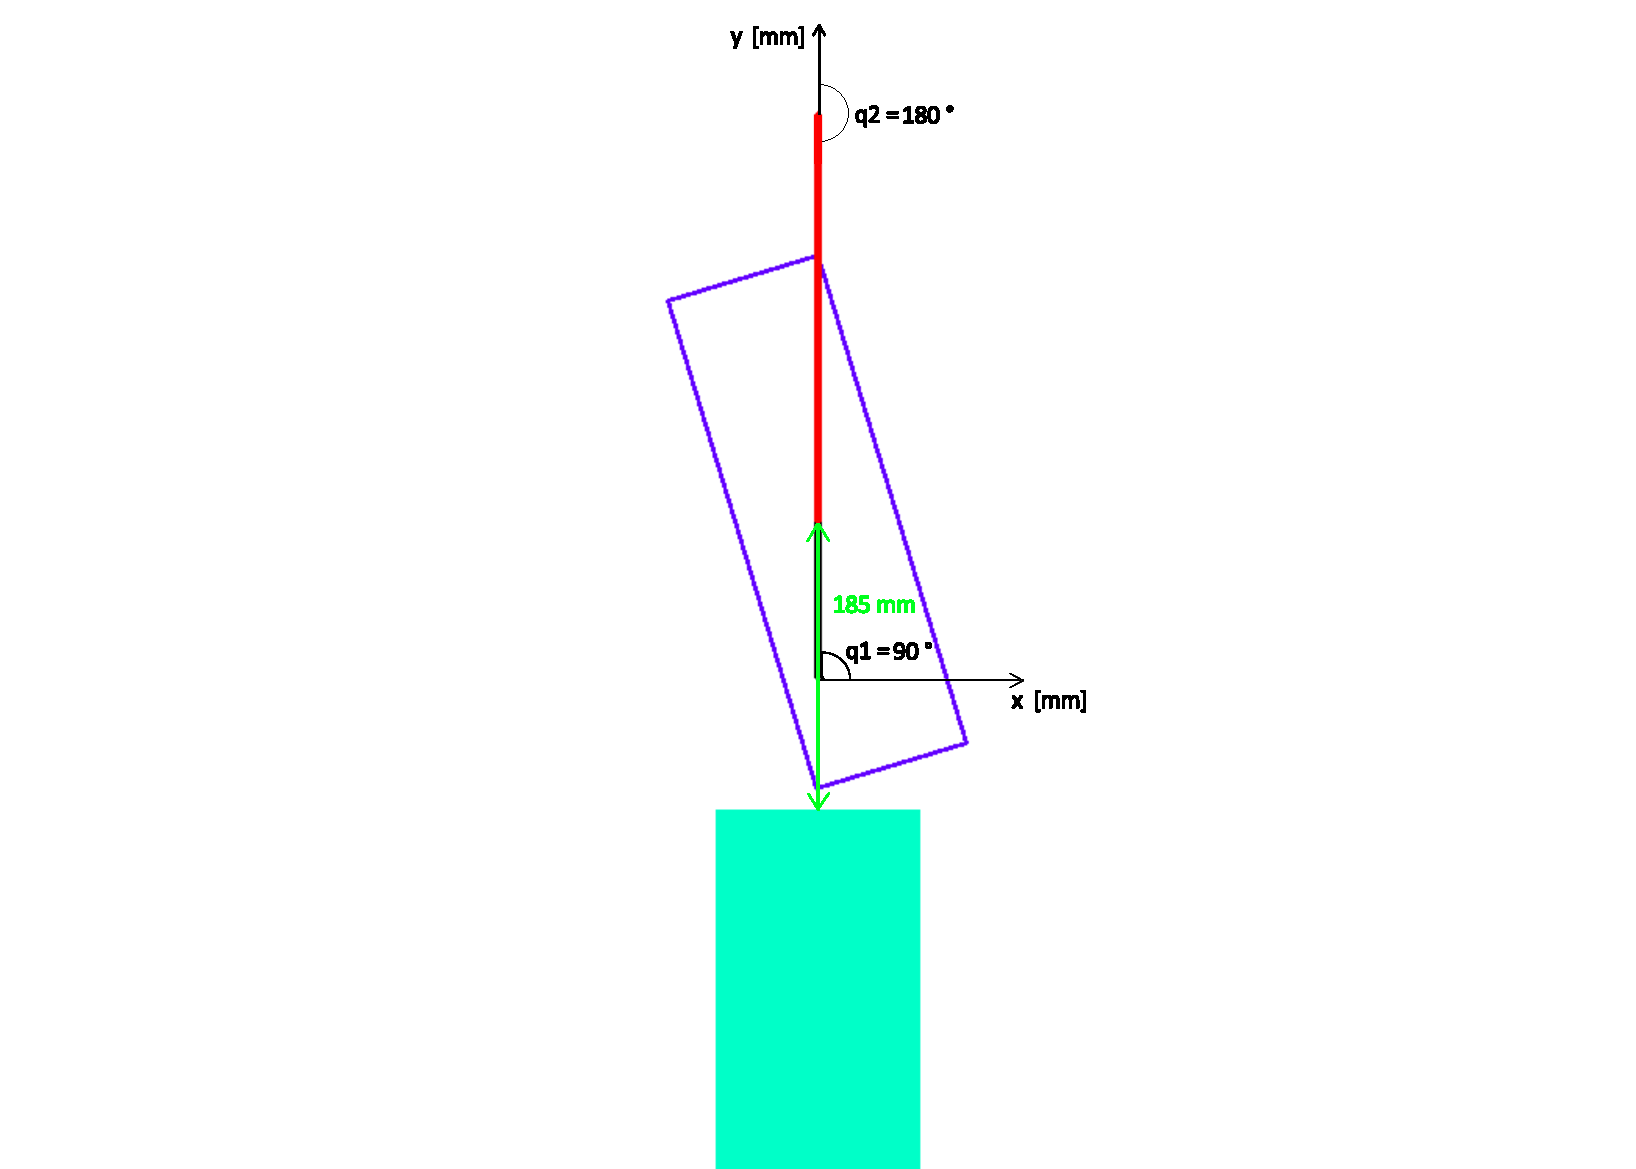
\includegraphics[width=160mm]{img/PREROT-uhlopriecka.pdf}
	\caption{ Hraničná situácia prechodu} \label{OBRAZOK 4.12} 
\end{figure} 

Druhým krokom je zistenie aká musí byť orientácia objektu aby bolo možné nájsť riešenie. Zároveň treba overiť či je táto orientácie dosiahnuteľná vrámci pracovného priestoru robotu.  
Na zistenie potrebnej orientácie objektu sme si vytvorili tvz. bezkolíznu kružnicu. Ide o pomyselnú kružnicu, ktorej stred sa nachádza v pozícii druhého rotačného kĺbu ramena pri konfigurácii  $ q_1 = 90 \degree $ a $ q_2 = 180 \degree $. Jej polomer je definovaný vzdialenosťou druhého kĺbu ramena od stĺpa v smere osi $ x $, čo sa rovná $ 445 mm $.  Ak sa všetky pozície rohov objektu nachádzajú pri danej konfigurácii v bezkolíznej kružnici vieme povedať, že objekt pri danej orientácii bude schopný obísť prekážku a teda dosiahnuť cieľovú konfiguráciu. Na obrázkoch \ref{OBRAZOK 4.13}  a \ref{OBRAZOK 4.14} môžeme vidieť ako orientácia toho istého objektu ovplyvní možnosť dosiahnutia cieľa. 


\begin{figure}[h]
	\centering
	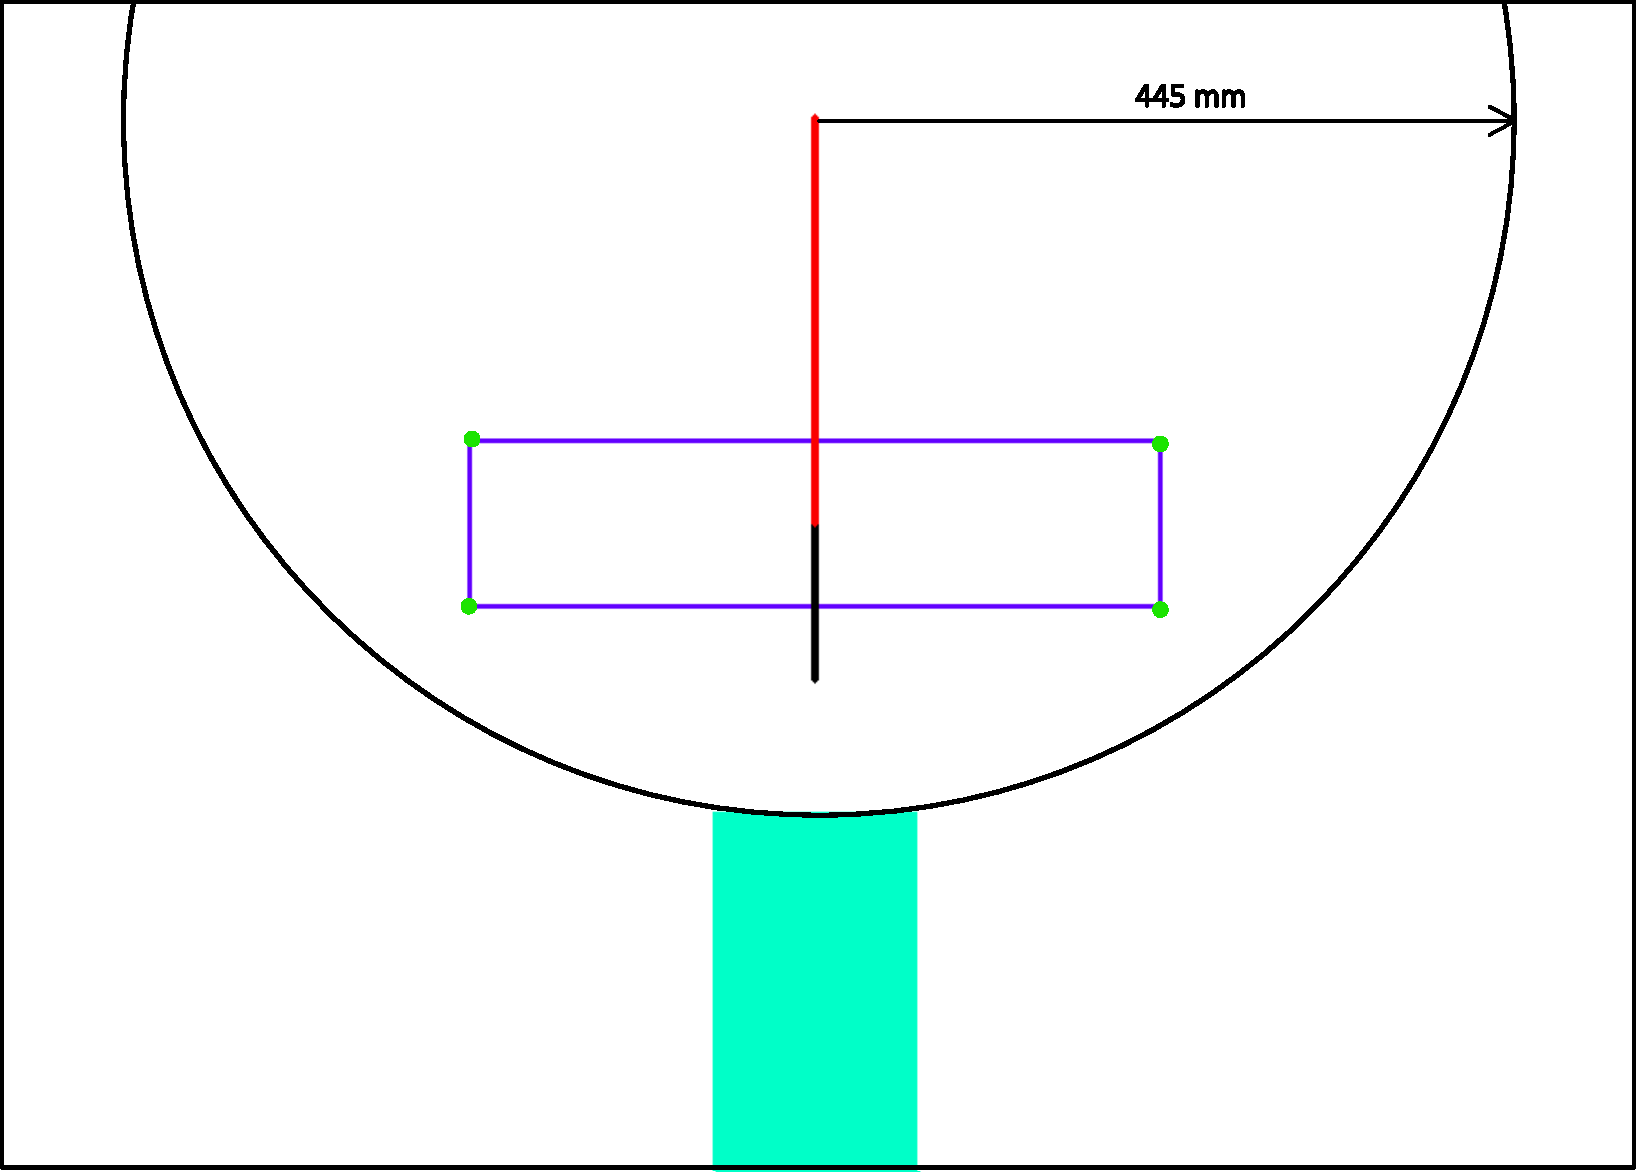
\includegraphics[width=90mm]{img/PREROT-kruznica2.pdf}
	\caption{ Bezkolízna kružnica - bezkolízny stav} \label{OBRAZOK 4.13} 
\end{figure} 

\begin{figure}[h]
	\centering
	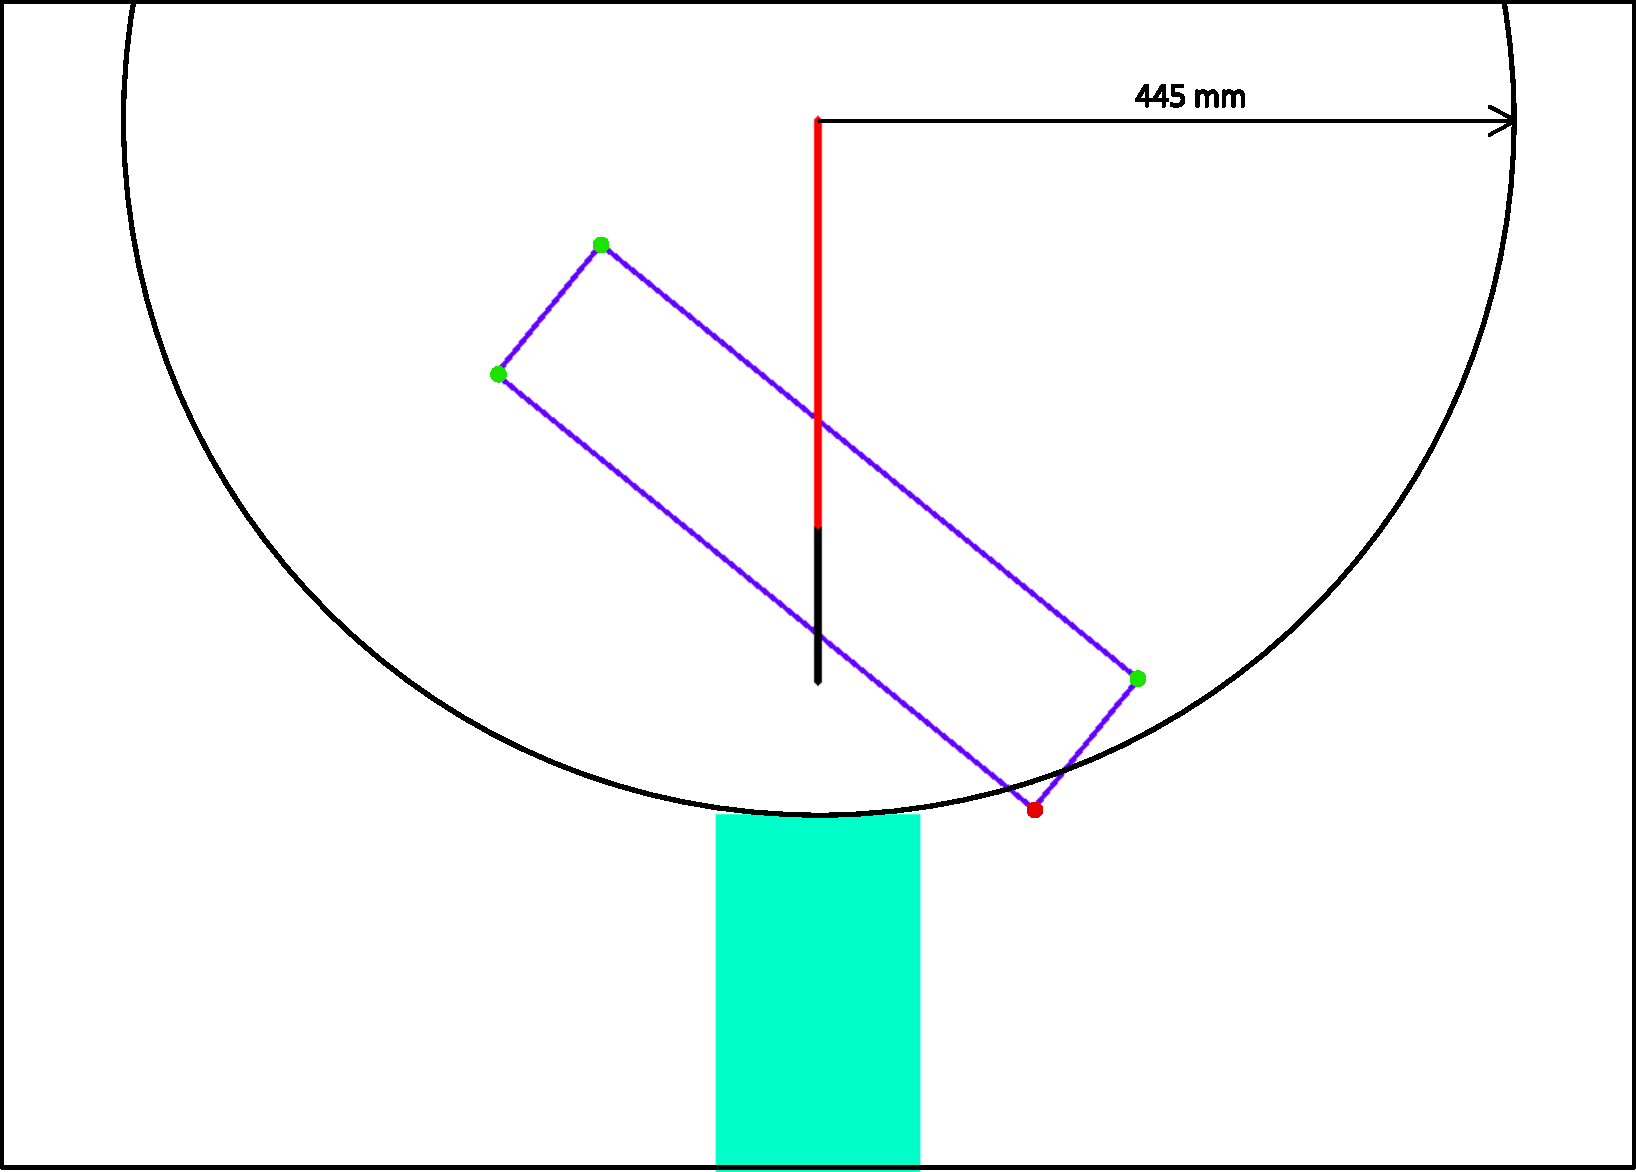
\includegraphics[width=90mm]{img/PREROT-kruznica1.pdf}
	\caption{ Bezkolízna kružnica - kolízny stav} \label{OBRAZOK 4.14} 
\end{figure} 
Proces hľadania tejto orientácie teda prebieha v nasledujúcich krokoch. Získame množinu všetkých dosiahnuteľných polôh v počiatočnej pozícii. Postupne inkrementujeme natočenie objektu v danej polohe a kontrolujeme, či sa nenachádza v kolízii. Podobne postupujeme aj v cieľovej pozícii. Následne tieto dve množiny porovnáme a získame ich prienik. To nám poskytne výslednú množinu orientácií objektu, v ktorých sa nebude nachádzať v kolízii v počiatku ani v cieli. Následne overíme v danej množine existuje konfigurácia, v ktorej by sa objekt nachádzal vo vnútri bezkolíznej kružnice. V prípade, že existuje takáto konfigurácia algoritmus si zapamätá aká musí byť orientácia v počiatočnom bode a po uchytení objektu je natočení do požadovanej orientácie. Následne je zavolaný RRT algoritmus, ktorého výstupom je výsledná trajektórie s už natočeným objektom.

\begin{figure}[h]
	\centering
	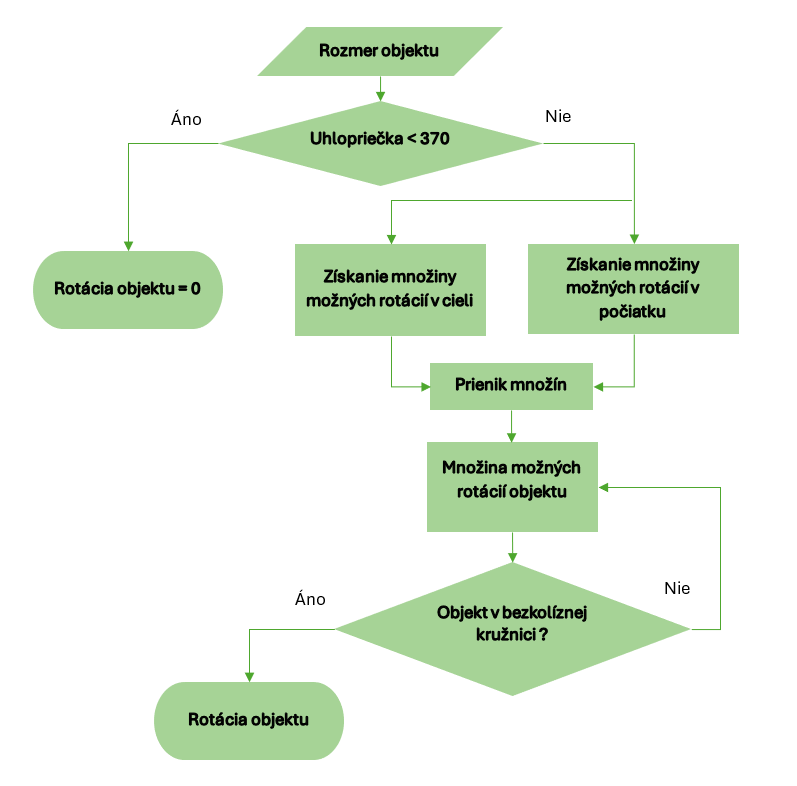
\includegraphics[width=140mm]{img/VD_predrot.png}
	\caption{ Princíp predrotácie} \label{OBRAZOK 4.15} 
\end{figure} 

